\chapter{Configuration du côté client}

Le côté client est une partie toute aussi importante que notre côté serveur parce qu'elle nous permet d'envoyer des paquets vers le serveur et vérifier si la configuration de notre protocole applicatif à fonctionner.

\subsection{Alternative possible avant de coder pour vérifier protocole applicatif}

Comme j'ai pu le dire précédemment, nous pouvons avant de coder notre côté client utiliser des utilitaires \textbf{permettant de vérifier} si notre protocole applicatif ne rencontre aucun souci 'visible' (car nous devrons envoyer l'ensemble de la requête à la main). \\ \par

Ce genre de manipulation peut avoir plusieurs \textbf{bienfait} mais aussi quelques \textbf{désavantages} : \\ \par

\boit{Avantages} :
\begin{itemize}
    \item Tester notre côté serveur au fur et à mesure sans devoir coder notre client en même temps
    \item Pouvoir détecter les erreurs
\end{itemize} \hfill \\ \par

\boit{Inconvénient} :
\begin{itemize}
    \item Problèmes de sécurité (car nous permettons une application tierce de se connecter)
    \item Pourrait trouver une faille dans le protocole et l'exploiter
    \item Il faut gérer les caractères de fin envoyé par certains protocole du côté serveur (CRLF qui correspond au caractères de fin de line (Carriage Return Line Feed))
\end{itemize} \hfill \\ \par

Voici à quoi ressemblerait une requête envoyé avec \textit{Telnet} vers le serveur :

    {
    \centering
    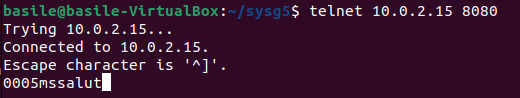
\includegraphics[width=18cm]{figures/example_telnet_conn.png}
    \par
    } \hfill \\ \par

Il faut bien évidemment donner l'adresse IP + le port à la commande :
\begin{lstlisting}
    telnet IpAdress Port
\end{lstlisting}

Nous encodons à la 'main' l'envoie du message mais contenant notre protocole vu que notre prochaine application fera ca pour nous tout à l'heure.

\subsection{Notre côté client, création socket}

Notre application devra se connecter à notre serveur pour cela, on devra comme le serveur de :
\begin{itemize}
\item Créant un point de communication (Socket)
\item Rentrer les informations du serveur dans une structure (sockaddr in) pour définir où et comment se connecter
\item Se connecter  au point de communication via Connect
\end{itemize}

\lstinputlisting{codes/createSocketClient.c} \hfill \\ \par

Nous utilisons des appels systèmes assez importants pour la connection. Bien évidemment certains d'entre eux, on déjà pu être vu comme : socket()

\begin{lstlisting}
    connect(socketfd,(SA*)&server_addr,sizeof(server_addr)
    Nous devons specifie a quel socket se connecter (c'est pour cela que nous avions 
    rentre les informations du serveur).
    En plus de ca, nous fournissons une structure qui permet de stocker 
    les informations de celui-ci.
\end{lstlisting} \hfill \\ \par

Nous pouvons commencer à envoyer si nous souhaitons des informations au serveur grâce à l'appel système : send() que nous verrons plus tard.

\subsection{Notre côté client, envoie de message}

Nous devons définir plusieurs choses avant de commencer à réaliser l'envoie de message. \\ \par

\begin{itemize}
\item Définir notre type d'envoie courant (soit un message (s) ou un fichier (f))
\item Définir le contenu d'envoie courant (si c'est le début, le milieu ou la fin comme défini dans le côté serveur)
\item Créer des fonctions qui retourne la taille d'un message et le stock (la partie code se trouve en annexe si besoin), et correspond à notre côté applicatif
\end{itemize}\hfill \\ \par

Une fois que tout ca est fait, nous pouvons passer à l'envoie de message via l'appel système \textbf{send} :
\begin{lstlisting}
send(socket, message, tailleMsg, flag)
Nous donnerons le socket stocke et renvoyer precedemment, le message contenant
notre protocole applicatif dedans et la taille de celui-ci.
Le flag ne nous interesse pas dans notre cas.
Voici un exemple :
send(socketfd, message, strlen(message),0)
\end{lstlisting}

Le 0 dans le flag est l'équivalent de donné aucun paramètre à notre fonction. \\ \par

Nous allons illustrer ca sous forme de dessin la sélection et l'envoie. \\ \\

\textit{Choisir le mode d'envoie qu'on souhaite} :

    {
    \centering
    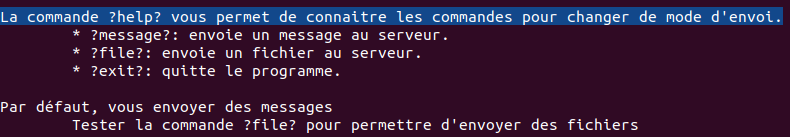
\includegraphics[width=18cm]{figures/selection_type_client.png}
    \par
    } \hfill \\ \par

    Si nous décidions de changer de \textbf{MODE} cela modifirait le type de contenu qu'on souhaite envoyé : \par
    \tab[2cm]Si notre type était avant et après:
    \begin{lstlisting}
        currentCommand='m' et qu'on souhaiterait changer vers l'envoie de fichier (qui se fera plus tard)
        currentCommand='f'
    \end{lstlisting}

    Il faudra bien évidemment vérifier si le serveur n'a pas eu de 'soucis' et à crasher ou vous a déconnecter. Pour cela, on utilise l'appel système : recv avec le flag MSG PEEK \\ \par

    On peut donc passer à la réel lecture au clavier...

    {
    \centering
    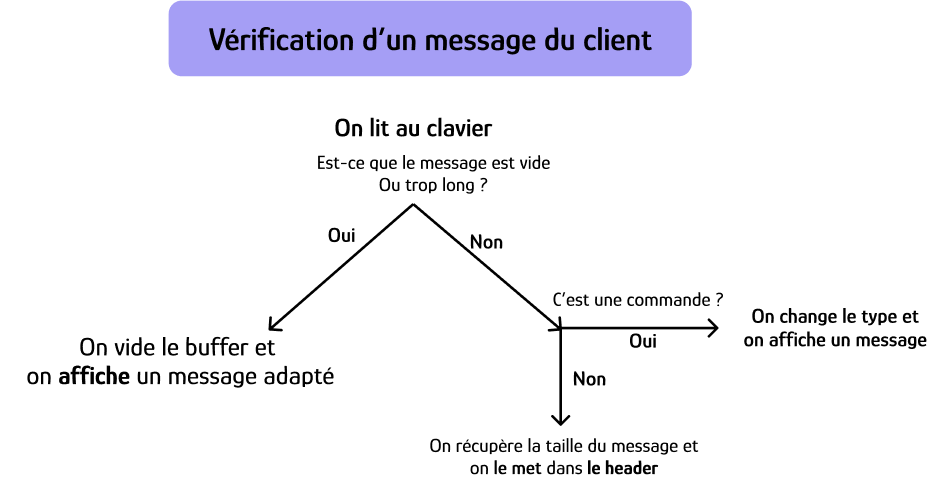
\includegraphics[width=14cm]{figures/verif_msg_client_send.png}
    \par
    } \hfill \\ \par

    Nous avons vérifier et implémenter une partie du header (les 4 bytes pour définir la taille du message), il nous reste simplement qu'à vérifier le \textbf{TYPE de message} qu'on souhaite envoyé et remplir le header pour matcher avec notre protocole applicatif. \\ \par

     {
    \centering
    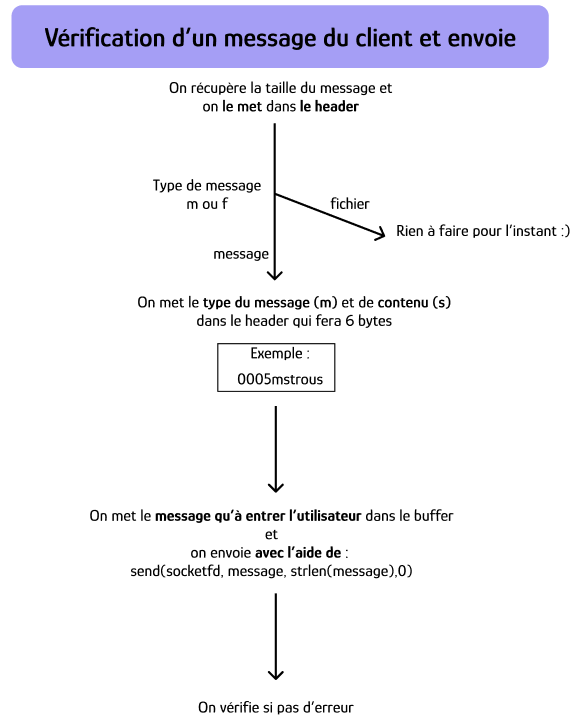
\includegraphics[width=11cm]{figures/verif_msg_client_next.png}
    \par
    } \hfill \\ \par

    Voila notre envoie de message fait en vérifiant les cas pouvant engendrer des erreurs. \\ \par\textbf{N'OUBLIEZ PAS, il est important de vérifier si un appel système à retourner une erreur}

\subsection{Notre côté client, envoie de fichier}

Comme précédemment dis, l'envoie de fichier ou bien même d'autres fonctionnalité sont de plus en plus développé. \\ \par

Un fichier est concrètement qu'un ensemble de bytes. Il suffit donc de récupérer ses bytes et les envoyés au fur et à mesure. \\ \par

Pour l'envoie de fichier, le schéma sera légérement modifiés à celui précédemment. \\ \par

Notre fichier qui sera envoyé aura des header différents en fonction de l'endroit ou ou se trouve :
\begin{itemize}
    \item Si on envoie notre nom de fichier. On enverra fs (fichier start)
    \item Si on envoie le contenu du fichir. On enverra fc (fichier continue)
    \item Si on est a la fin du fichier (pour pouvoir au serveur d'enregistrer le fichier). On enverra fe (fichier end)
\end{itemize}

    {
    \centering
    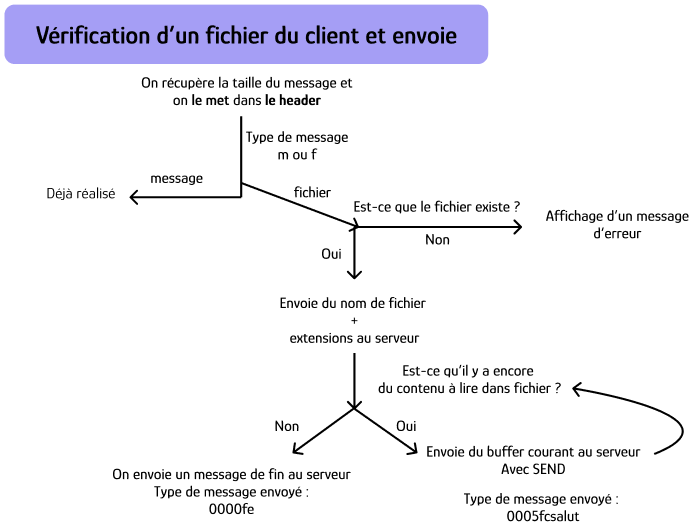
\includegraphics[width=13cm]{figures/verification_fichier_client_envoie.png}
    \par
    } \hfill \\ \par

    Comme dis au dessus, nous passons par des phases dans l'envoie du fichier vers notre côté serveur. Permettant à notre serveur, de savoir à quel endroit nous sommes dans notre fichier.

    Voici la fin de notre côté client qui permet un protocole applicatif plus ou moins riches en fonctionnalité et permet de vérifier les erreurs.